%  article.tex (Version 3.3, released 19 January 2008)
%  Article to demonstrate format for SPIE Proceedings
%  Special instructions are included in this file after the
%  symbol %>>>>
%  Numerous commands are commented out, but included to show how
%  to effect various options, e.g., to print page numbers, etc.
%  This LaTeX source file is composed for LaTeX2e.

%  The following commands have been added in the SPIE class
%  file (spie.cls) and will not be understood in other classes:
%  \supit{}, \authorinfo{}, \skiplinehalf, \keywords{}
%  The bibliography style file is called spiebib.bst,
%  which replaces the standard style unstr.bst.

\documentclass[]{spie}  %>>> use for US letter paper
%%\documentclass[a4paper]{spie}  %>>> use this instead for A4 paper
%%\documentclass[nocompress]{spie}  %>>> to avoid compression of citations
%% \addtolength{\voffset}{9mm}   %>>> moves text field down
%% \renewcommand{\baselinestretch}{1.65}   %>>> 1.65 for double spacing, 1.25 for 1.5 spacing
%  The following command loads a graphics package to include images
%  in the document. It may be necessary to specify a DVI driver option,
%  e.g., [dvips], but that may be inappropriate for some LaTeX
%  installations.
\usepackage[]{graphicx}
\usepackage{amssymb}
\graphicspath{{pics/}}

\usepackage{tabularx}
\renewcommand{\tabularxcolumn}[1]{>{\arraybackslash}m{#1}}

\title{A Framework for Automatic Tuning of System Parameters and Its Use in Image Registration}

%>>>> The author is responsible for formatting the
%  author list and their institutions.  Use  \skiplinehalf
%  to separate author list from addresses and between each address.
%  The correspondence between each author and his/her address
%  can be indicated with a superscript in italics,
%  which is easily obtained with \supit{}.

\author{Ren Hui Gong\supit{a} and Ziv Yaniv\supit{a}
\skiplinehalf
\supit{a}Sheikh Zayed Institute for Pediatric Surgical Innovation, Children's National Medical Center, Washington, DC 20010, USA
}

\authorinfo{E-mail: \{rgong,zyaniv\}@cnmc.org}

%>>>> Further information about the authors, other than their
%  institution and addresses, should be included as a footnote,
%  which is facilitated by the \authorinfo{} command.

%\authorinfo{Further author information: (Send correspondence to A.A.A.)\\A.A.A.: E-mail: aaa@tbk2.edu, Telephone: 1 505 123 1234\\  B.B.A.: E-mail: bba@cmp.com, Telephone: +33 (0)1 98 76 54 32}
%%>>>> when using amstex, you need to use @@ instead of @


%%%%%%%%%%%%%%%%%%%%%%%%%%%%%%%%%%%%%%%%%%%%%%%%%%%%%%%%%%%%%
%>>>> uncomment following for page numbers
% \pagestyle{plain}
%>>>> uncomment following to start page numbering at 301
%\setcounter{page}{301}

\begin{document}
\maketitle

%%%%%%%%%%%%%%%%%%%%%%%%%%%%%%%%%%%%%%%%%%%%%%%%%%%%%%%%%%%%%
\begin{abstract}
The performance of most segmentation and registration algorithms depends on the values of internal parameters.
Most often, these are set empirically. This is a trial-and-error process in which the developer modifies the values in an attempt to improve performance. This is an implicit form of optimization. In this paper, we present a more \emph{intuitive} and \emph{systematic} framework for this type of problem. We then use it to estimate optimal parameter values of a common registration problem. We formulate the performance of the registration problem as a function of its internal parameters, and use optimization techniques to search for an optimal value for these parameters. Registration quality is evaluated using a set of training images in which the anatomy of interest was segmented and comparing the overlap between the segmentations as induced by the registration. As a large number of computationally complex registrations are performed during the optimization, a cluster of MPI-enabled computers are used collaboratively to reduce the computation time. We evaluated the proposed method using ten CT images of the liver from five patients, and evaluated three optimization algorithms. The results showed that, compared with the empirical values suggested in the published literature, our technique was able to obtain parameter values  that are tuned for particular applications in a more intuitive and systematic way. In addition, the proposed framework can potentially be used to tune system parameter values appropriate for specific input types.
\end{abstract}

%>>>> Include a list of keywords after the abstract

\keywords{parameter tuning framework, meta-optimization, image registration, MPI-based computation}

%%%%%%%%%%%%%%%%%%%%%%%%%%%%%%%%%%%%%%%%%%%%%%%%%%%%%%%%%%%%%
\section{Motivation}

Nearly every computational system in medicine, software or hardware, has internal parameters, and the settings of the parameter values are critical to the system's overall performance. While there are well established methods to determine the parameter values for systems with analytical models (e.g. calibration parameters for imaging devices), empirical approaches through trial-and-error are commonly adopted for the majority of other parameters (e.g. parameters in image registration that are involved in image pre-processing, similarity metric definition, function optimization, and so on). One main disadvantage of empirical approaches is that the obtained parameter values are arbitrary, and we may not even know whether they are optimal or not including for the training set on
which they were assessed. In clinical practice, ideal parameter values can differ greatly even for similar tasks such as registration of different bony structures. Fine-tuned parameters can potentially improve the performance of these applications.

In this paper, we propose a framework to automate the process of parameter tuning, and use it to refine several numerical\footnote{A system can have non-numerical or discrete parameters that are critical; however, they are beyond the scope of this work.} parameters of a common registration problem. This approach uses optimization techniques to improve the settings of system parameter values, and requires intuitive user inputs to drive the search. Thus, it provides a more systematic and resilient approach for a large number of similar problems.
As we are designing a generic framework, we are not guaranteed that the optimized function is convex, nor that it
is smooth, making optimization a challenging task. An additional potential challenge has to do with the computational complexity of the function evaluation, in some cases this can be prohibitive and would benefit from the use of a distributed computing framework.

Our approach to optimizing the parameters involved in registration can be viewed as a variant of meta-optimization~\cite{metaopt}. That is, we use optimization techniques to obtain optimal parameter values for other optimization methods. This approach has been previously applied to tuning neural networks, and various evolutionary algorithms~\cite{smit09:ece}. In this work, we aim to provide a general framework for problems in the medical domain and address the associated challenges.

%%%%%%%%%%%%%%%%%%%%%%%%%%%%%%%%%%%%%%%%%%%%%%%%%%%%%%%%%%%%%
\section{Method}

\subsection{General Framework for System Parameters Tuning}

The performance of a parametric computational system depends on two things: the \emph{internal parameter value} settings and the user-supplied \emph{input}. We represent such systems using a vector of parameters $p$, and an abstract data structure $data$. Usually, the internal parameters are fixed or user-configurable within a predefined range when the system is deployed, while the data being processed during
production can have a large variability and the outcome is highly dependent on the settings of the internal parameters. In this work, we only consider parameters in $\mathbb{R}$ that can be numerically optimized, although other types of parameters may also be important to the system.

Assume that, for any given setting of the parameters and any given user data, we are given a function $f$ which reflects the system performance. The problem of parameter tuning is formulated as an optimization of the function $f(p,\{data\})$ with respect to parameters $p$, taking into account all possible variability of the user data. Using this formulation we assume that as input we are given training data, denoted $\{data\}_i, i=1...N$, that captures the distribution of the expected inputs. That is, given a user provided function, $f$, and a training data set, $\{data\}$, we automatically estimate the optimal parameter values for the system. Fig.~\ref{fig:spt_framework} illustrates the main components as well as the flowchart of the framework we have developed.

\begin{figure}[tb!]
\begin{center}
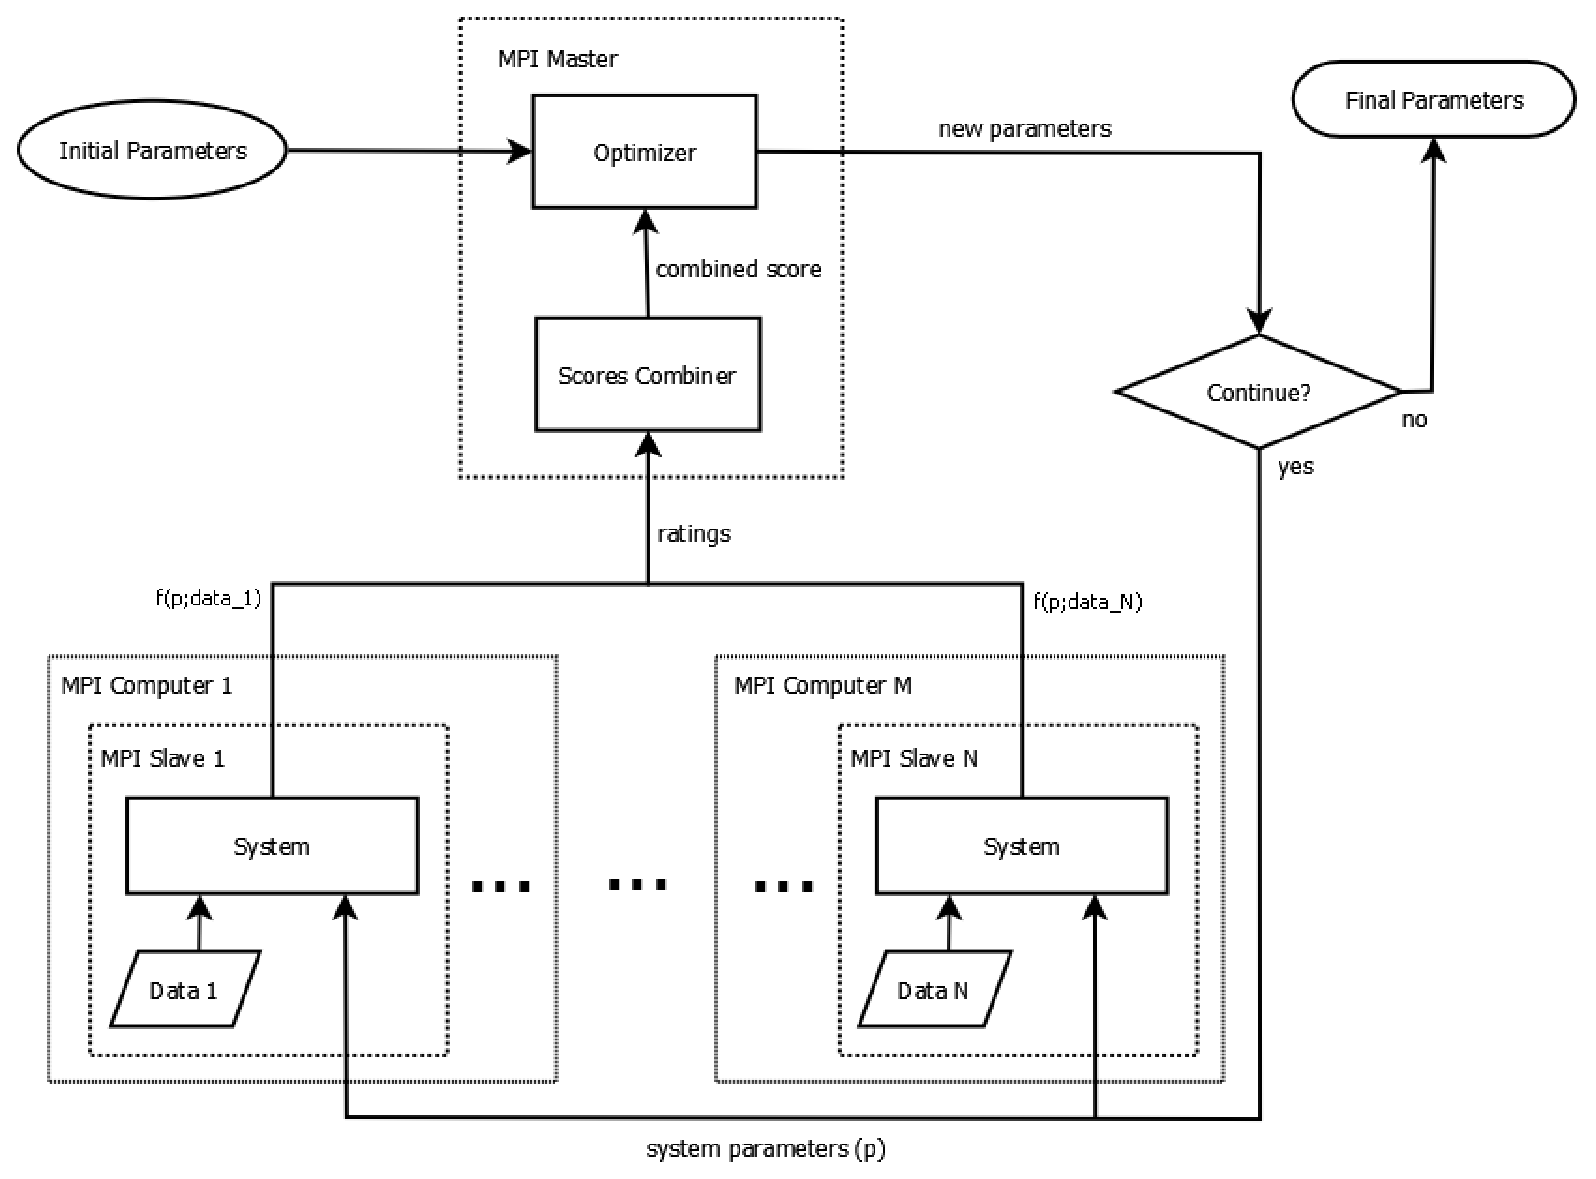
\includegraphics[width=5in]{framework}
%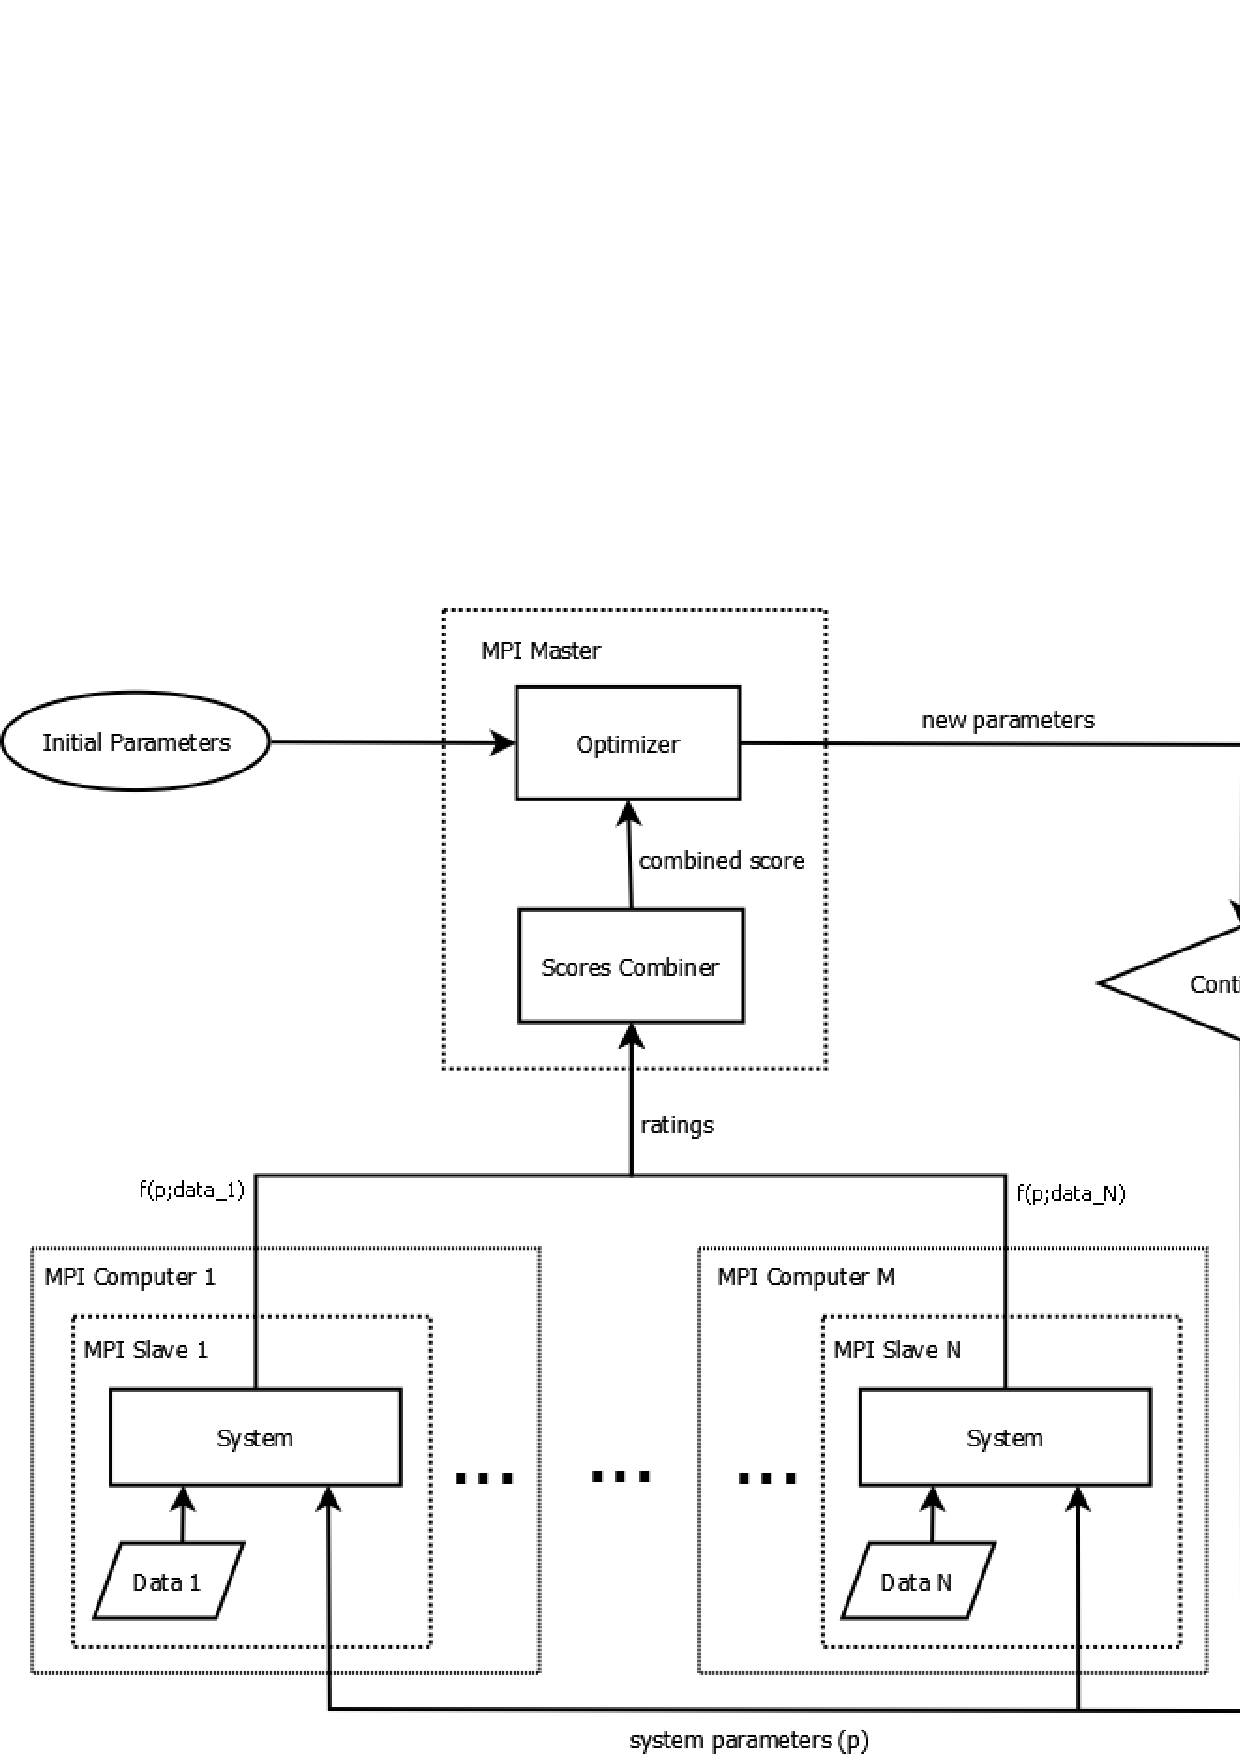
\includegraphics[trim=0cm 8cm 0cm 0cm, clip=true, width=5in]{framework.jpg}
\end{center}
\caption{General framework for system parameters tuning.}
\label{fig:spt_framework}
\end{figure}

In Fig.~\ref{fig:spt_framework}, an initial value of the parameters is provided to start the optimization process. In each optimization iteration, the parameters are fed into a set of $N$ instances of the system, each processes one training data set and is rated under the current setting of the parameters. The individual ratings are then collected and aggregated by a score combiner, which is in turn fed into the optimizer to produce an improved setting of the parameters.

In practice, the computation cost of this framework can be very high. This is mainly because it is often difficult to find a well-behaved function between the parameters and the system's overall performance, thus $f$ can be highly non-linear and very noisy. We thus turn to population-based optimization algorithms which are more appropriate for searching these types of functions. In addition, as we require that our training data represent the population variability its size is potentially very large. As a consequence, a single evaluation of
the function $f$ for a given set of parameters will have a high computational cost. To overcome these challenges, we propose to implement the framework on a cluster of workstations using the Message Passing Interface (MPI) \cite{SkjellumAn1994b}. As illustrated in Fig.~\ref{fig:spt_framework}, the problem is solved using a master-slave computing model on a set of $M$ computers. The function evaluation for each training data set is evaluated in a separate slave process, and the master process is responsible for combining the individual ratings and performing the optimization. Each participating computer can simultaneously run a number of slave processes that are specified by the user.

The type of user data, definition of the function $f$, choices of the optimizer, and so on, are application specific. In the next subsection, we present how this framework fits into the context of a common medical image processing task, registration.

\subsection{Optimization algorithms}

In general, the optimized cost function may not be smooth or convex,
rendering local optimization techniques such as the Nelder-Mead downhill
simplex method and GD unreliable. We use population-based optimization
algorithms to search for an optimal value for $p$. We evaluate three
algorithms, Particle Swarm Optimization (PSO) \cite{Kennedy95:NN}, Covariance
Matrix Adaptation Evolution Strategy (CMA-ES) \cite{Hansen06}, and an adapted
Brute-Force (BF) search. The PSO algorithm is a stochastic global search
optimization approach. Optimization is performed by maintaining a swarm of
particles that traverse the parameter space, searching for the optimal
function value. Associated with each particle are its location, speed, and
the location and value of the best function value it previously evaluated. A
particle's next location is determined by these values and the location of
the best function value evaluated by the swarm. The algorithm is initialized
using a uniform distribution over the user supplied feasible region. The
CMA-ES algorithm starts from an initial guess of the solution and an initial
search distribution that is centered at the initial guess. The search
distribution is represented using a multi-variate normal distribution, whose
initial shape is a sphere. In each evolution step, a small number of samples
are generated from the search distribution; then, the samples are selected
and combined, and the search distribution is updated accordingly. For our
adapted Brute-Force approach, we start by overlaying a uniform grid onto the
user supplied feasible region. The function is evaluated at all grid
locations and we select the location that has the best value. We then use
this solution as the initial input to a standard optimization algorithm. In
our case we use the downhill simplex method.

%The first two algorithms use a number of sample points in the parameter's space to drive the search process, thus they are more robust to noise and local minima. For the brute force approach, we first evaluate the function at points of a regular grid sampled from a user-defined region in the parameter's space; then, starting from the best value, a second search with the downhill simplex optimization algorithm is performed.

%PLEASE ELABORATE A BIT MORE ON THE ALGORITHMS.
%THE BOUNDING REGION FOR THE PSO DEFINES THE FEASIBLE SPACE, I BELIEVE THE CMA-ES HAS R^N (N - NUMBER OF PARAMETERS) AS THE FEASIBLE SPACE. ALSO THERE IS A DIFFERENCE BETWEEN BRUTE FORCE AND THE ADAPTED BRUTE FORCE. IN BF THE GRID IS OVERLAID ONTO THE  FEASIBLE REGION, WHILE THE ADAPTED BF HAS R^N AS THE FEASIBLE REGION.
%ALSO, THE USER SPECIFIES THE FEASIBLE REGION IN THE FRAMEWORK.
%FINALLY, ALGORITHM INITIALIZATION:PSO - PARTICLES UNIFORMLY DISTRIBUTED INSIDE FEASIBLE REGION. ADAPTED BF - UNIFORM GRID OVER THE FEASIBLE REGION. CMA-ES - HOW?


\subsection{Automatic Tuning of Registration Parameters}

\subsubsection{Parameters to be optimized}

Deformable 3D/3D (CT/CT) image registration is a fundamental task in medical image processing. It is commonly used for constructing anatomical atlases, and enabling image-guided interventions in soft tissue structures. The registration task is usually solved using a multi-level scheme: in the first level, the global alignment between the images is estimated using a transformation having a few degrees-of-freedom (DOFs) such as rigid, similarity or affine; in the second level, registration is locally refined with a transformation of higher DOFs such as Free Form Deformations (FFD). Gradient-descent (GD) is commonly used as the optimization algorithm in both levels because of its high efficiency. However, the settings of several internal parameters in GD can significantly affect the overall performance of the registration, which includes failure rate, accuracy, and computation time.

We use our framework to determine four critical parameters of GD for a typical deformable registration problem, which consists of a similarity registration in the first level, and a B-spline FFD registration in the second level.
The similarity registration determines three types of transformation parameters, which are rotation in the form of a versor, translation, and isotropic scaling. As the parameters are not commensurate it is common to scale their values so that changes in all values have similar effects on the change in the optimized function value. These scaling factors have a significant effect on the registration optimization process. If not set appropriately, the optimization may be biased to a subset of the transformation parameters, which yields premature termination or higher failure rate.
In the B-spline deformable registration, one important GD parameter is the relaxation factor, which determines how much or how fast to relax the step length when the current step length no longer drives the registration. Too large or too small step sizes will affect the registration performance, especially the convergence speed.
We use the following vector to represent the GD parameters to be optimized:
\begin{equation}
p = \{s_{v},s_{t},s_{s},r\},
\end{equation}
where $s_{v}$, $s_{t}$ and $s_{s}$ are the scaling factors for the components of rotation (i.e. versor), translation and isotropic scaling, respectively, in the similarity registration, and $r$ is the relaxation factor for the step length in the B-spline deformable registration.

We use the Insight Registration and Segmentation Toolkit (ITK)\cite{itk:v2.4} to implement this registration. There are suggested values for $p$ given in the ITK manual and examples; however, no reasoning is given with regard to the specific value choices, and we do not know whether they are optimal in some sense.

\subsubsection{Evaluation of registration performance}

The performance of the described registration is evaluated by performing a number of registrations with a set of training images and evaluating the overall final alignment.

For each training image, an anatomy of interest is pre-segmented. The final alignment of a registration is calculated as the complement of the Dice Similarity Coefficient (DSC) \cite{dsc}, which computes the ratio of overlap between the two segmentations. The complemented DSC for a pair of images $(I^A_i, I^B_i)=data_i$ is defined as follows:
\begin{equation}
f(p; I^A_i, I^B_i) = 1.0 - \frac{2.0 \times \vert S^A_i \bigcap R(p,S^B_i) \vert}{\vert S^A_i \vert + \vert R(p,S^B_i) \vert},
\end{equation}
where ($S^A_i$, $S^B_i$) are the corresponding segmentations, $R(p,.)$ denotes the registered image under parameters $p$, $\bigcap$ is the overlap between two segmentations, and $\vert . \vert$ denotes the number of voxels inside a segmentation or the overlap.

The overall final alignment is computed as the average alignment across all registrations:
\begin{equation}\label{eq:f_mean}
f(p; \{I^A_i, I^B_i\}_{i=1...N}) = \frac{1}{N}\sum^N_{i=1} f(p; I^A_i, I^B_i).
\end{equation}


%%%%%%%%%%%%%%%%%%%%%%%%%%%%%%%%%%%%%%%%%%%%%%%%%%%%%%%%%%%%%
\section{Results}

\subsection{Testing Data}

\begin{figure}[t!]
\begin{center}
\begin{tabular}{c|c|c|c|c|c}
%\begin{tabularx}{\textwidth}{X|X|X|X|X|X}
\hline
 & Patient 0 & Patient 1 & Patient 2 & Patient 3 & Patient 4 \\
\hline
Resolution & $512^2 \times 136$ & $512^2 \times 120$ & $512^2 \times 151$ & $512^2 \times 120$ & $512^2 \times 160$ \\
\hline
Spacing ($mm^3$) & \multicolumn{5}{c}{$0.976562^2 \times 2.5$} \\
\hline
T0 & 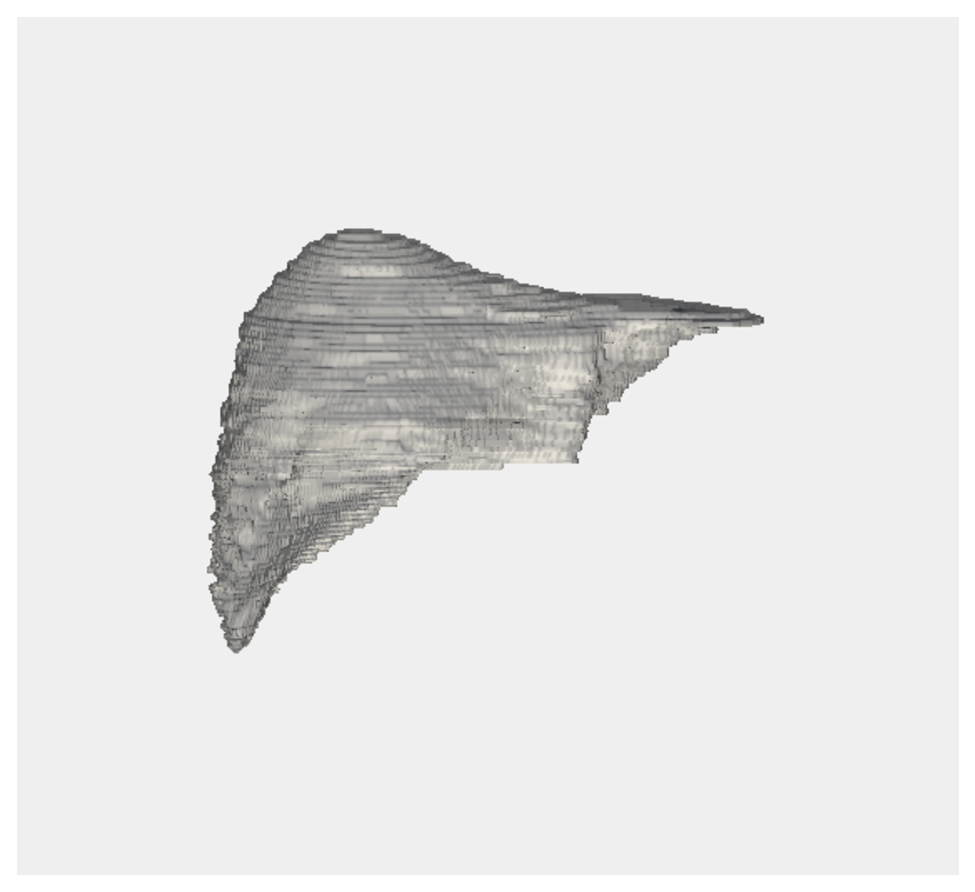
\includegraphics[width=0.7in]{seg_p0t0} & 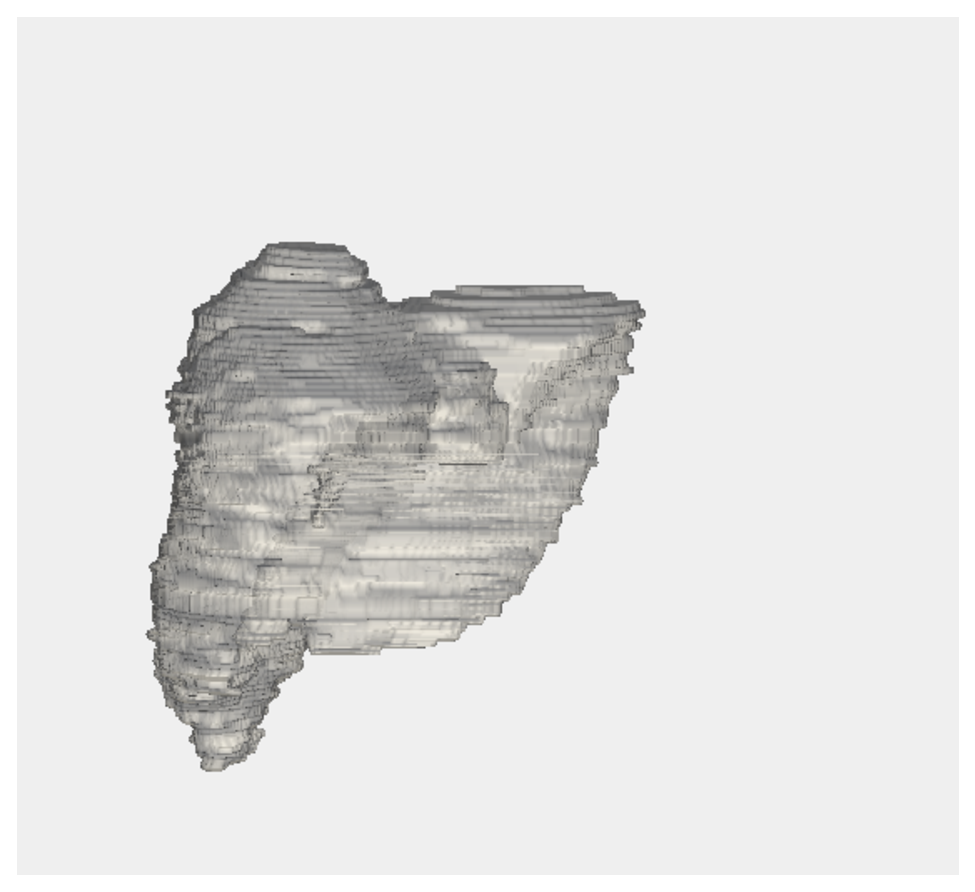
\includegraphics[width=0.7in]{seg_p1t0} & 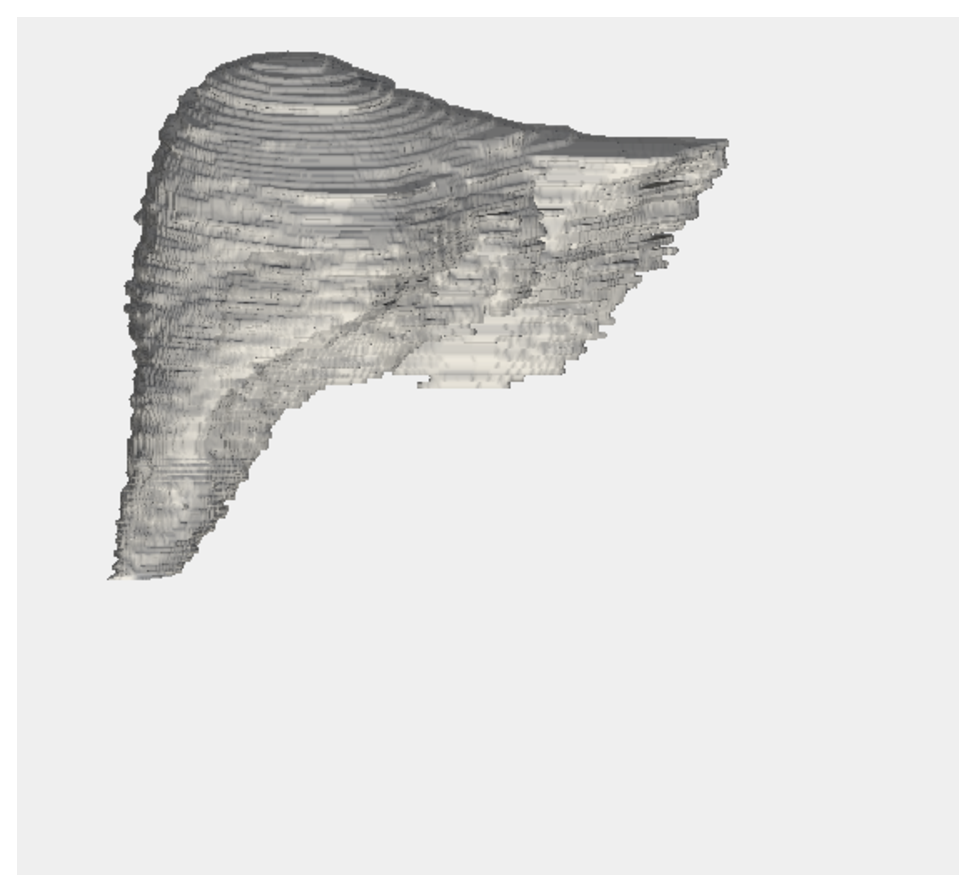
\includegraphics[width=0.7in]{seg_p2t0} & 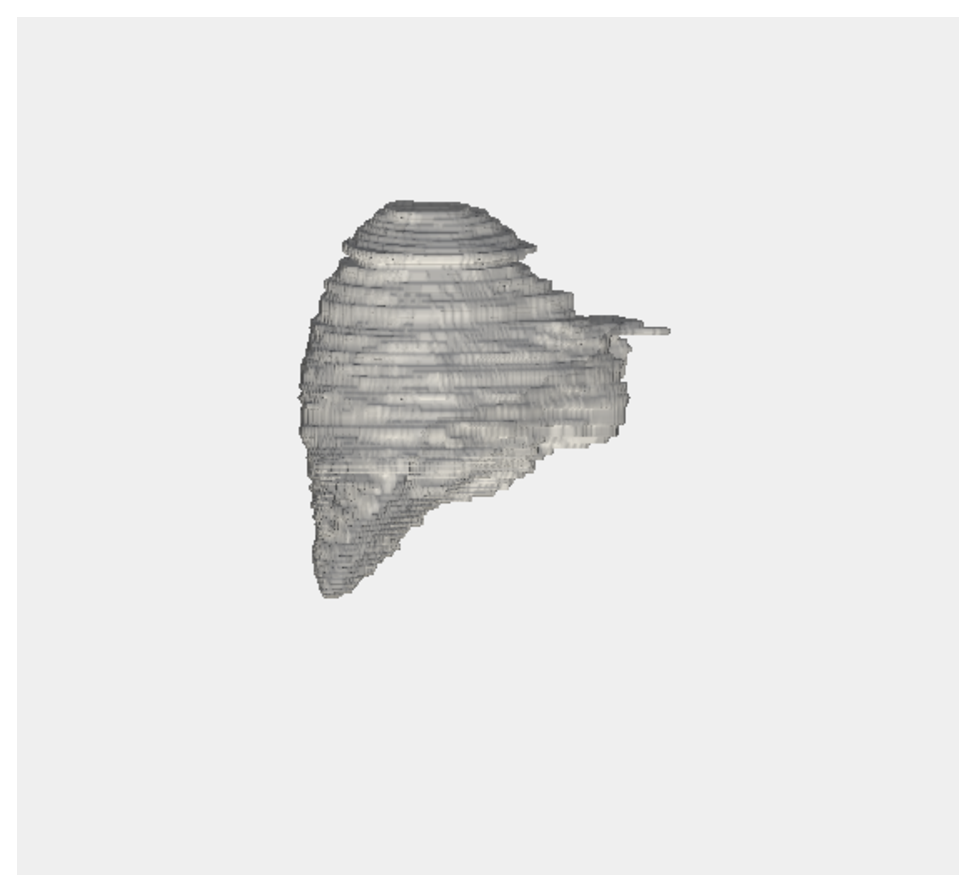
\includegraphics[width=0.7in]{seg_p3t20} & 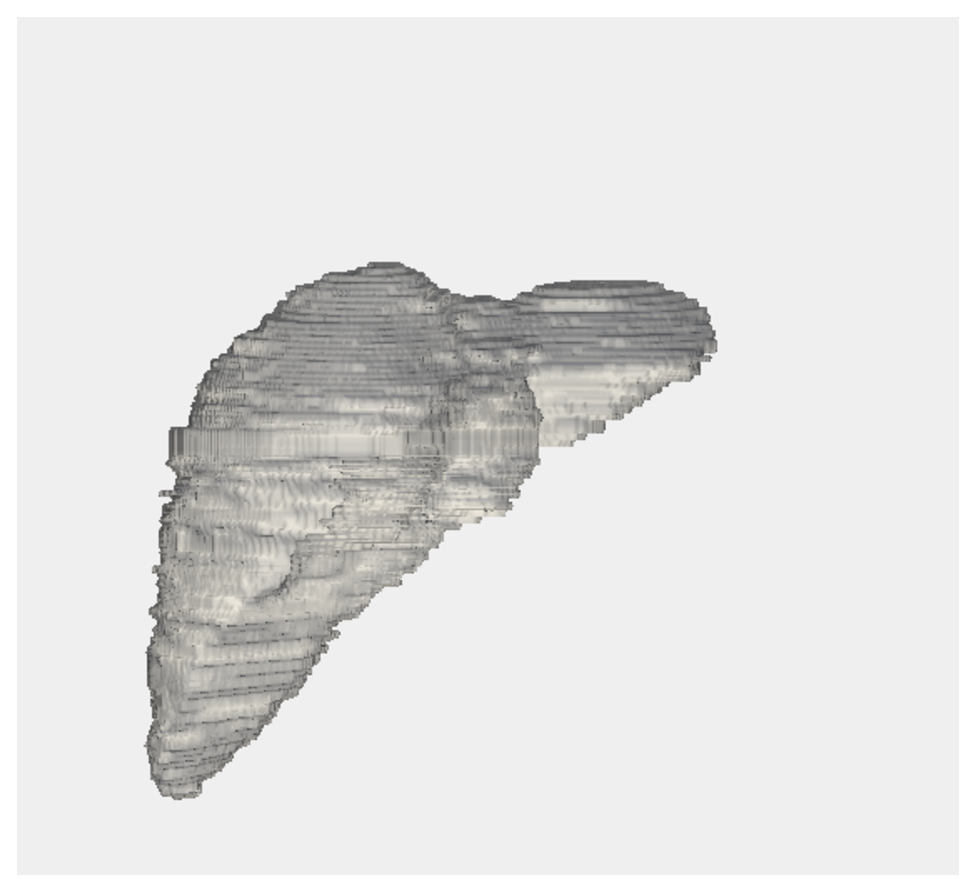
\includegraphics[width=0.7in]{seg_p4t0} \\
\hline
T50 over T0 & 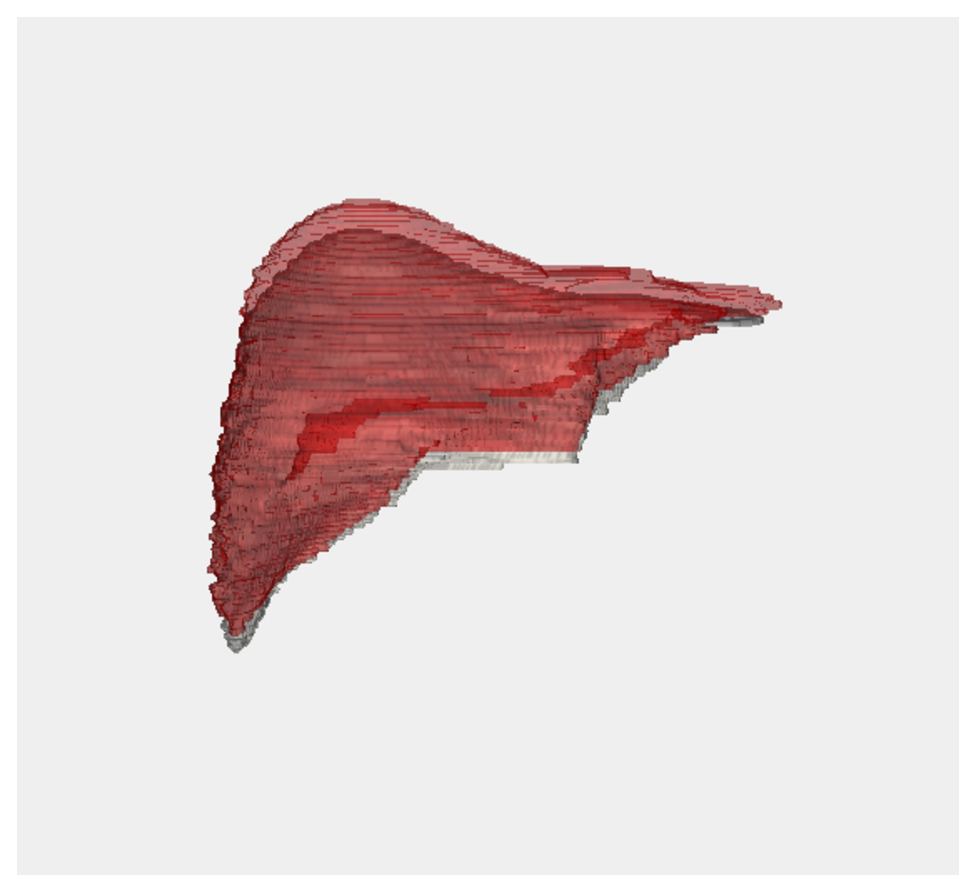
\includegraphics[width=0.7in]{seg_p0t0_t50} & 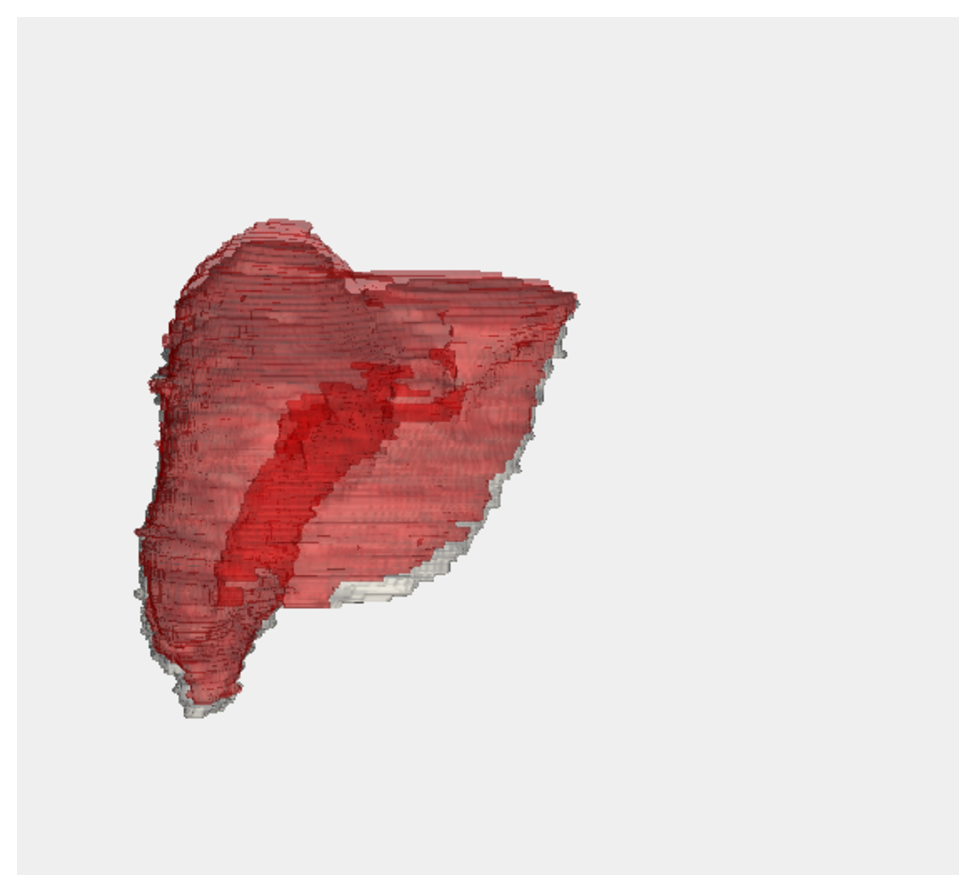
\includegraphics[width=0.7in]{seg_p1t0_t50} & 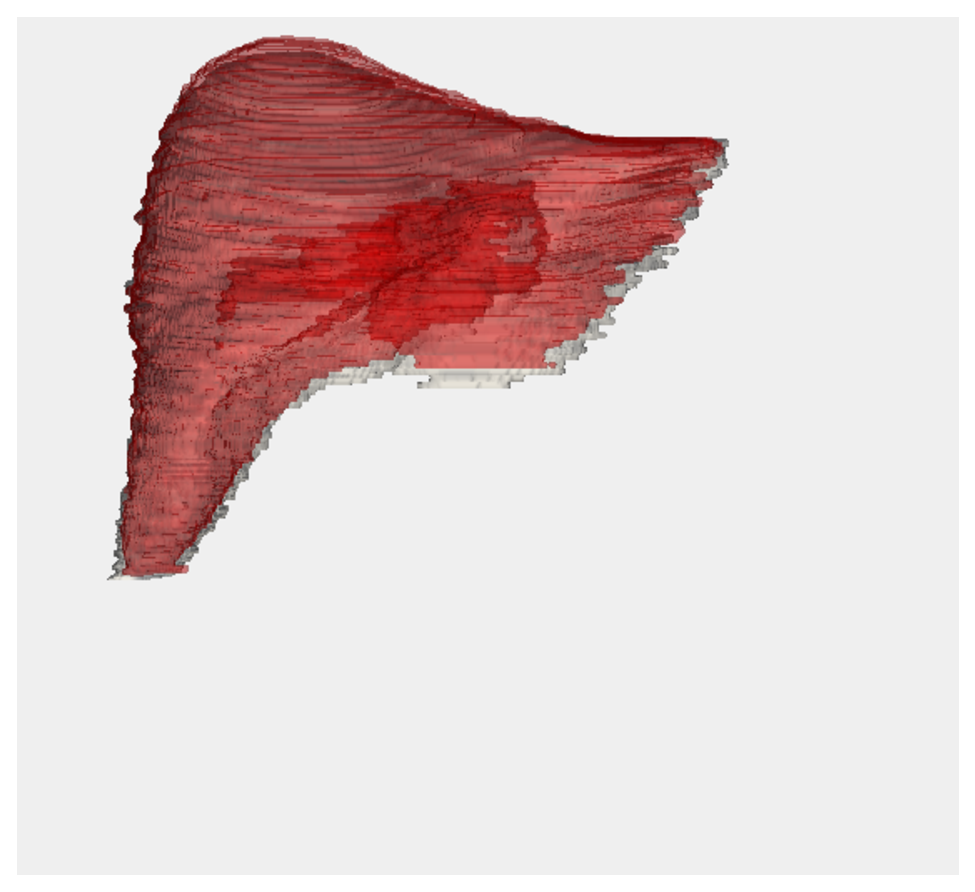
\includegraphics[width=0.7in]{seg_p2t0_t50} & 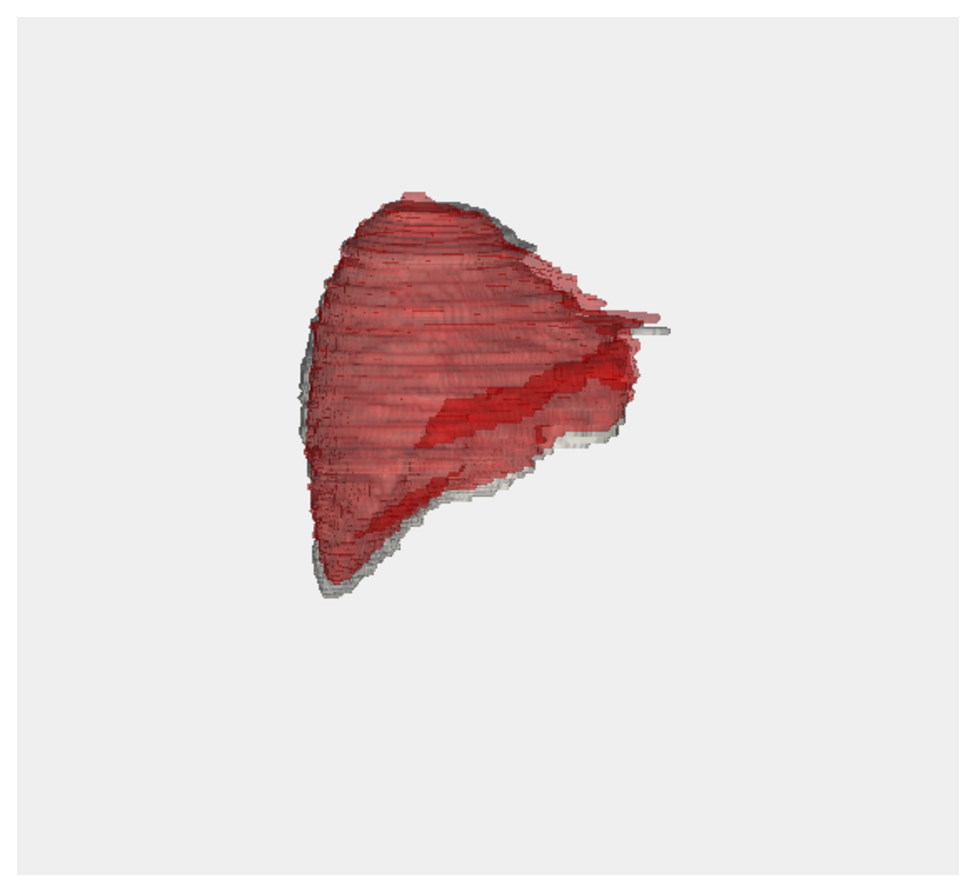
\includegraphics[width=0.7in]{seg_p3t20_t50} & 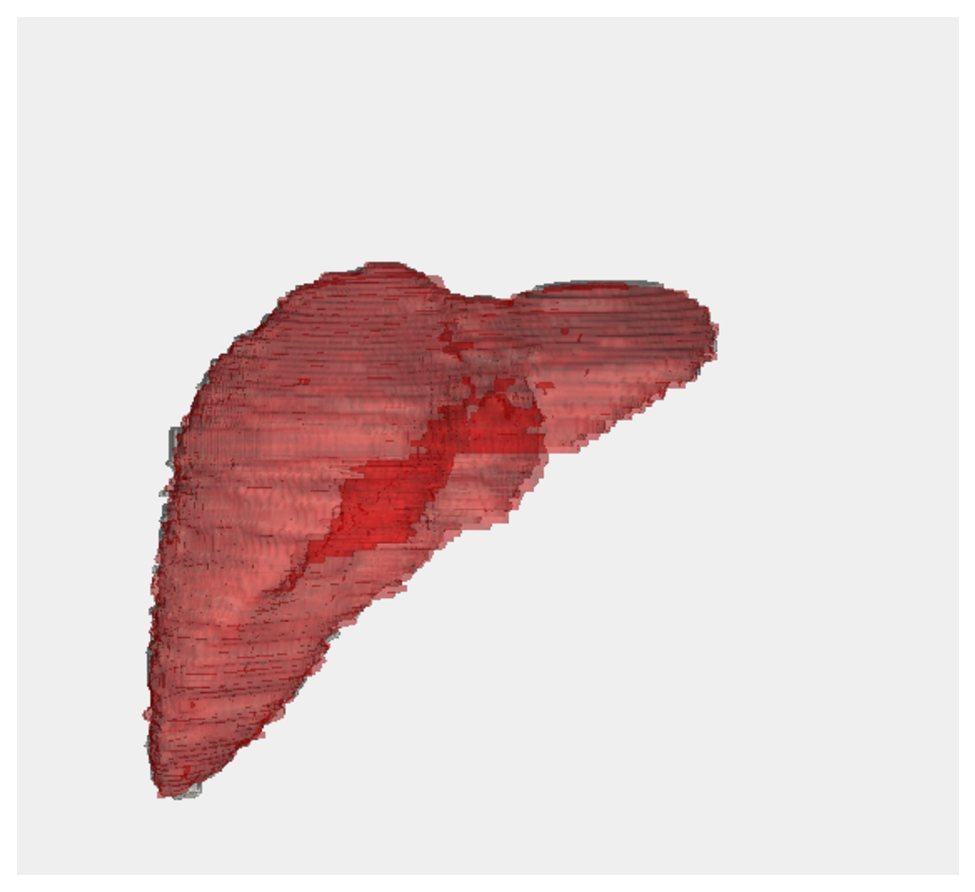
\includegraphics[width=0.7in]{seg_p4t0_t50}
\\
\hline
\end{tabular}
\vspace*{5mm}
\caption{Image specifications and coronal views of the segmented liver. The last row shows the overlaps between T0 (end-inhale) and T50 (end-exhale), which illustrates the largest motions between the two respiratory phases).}
\label{tab:data_specs}
\end{center}
\end{figure}

We used 4D CT abdominal images to evaluate the proposed method. The images came from five patient data sets, each consisting of ten CT images corresponding to different respiratory phases. We used two images from each patient, end-inhale\footnote{For patient 3, we used the first respiratory phase after end-inhale instead of end-inhale as the reconstruction of end-inhale exhibited large motion artifacts.} and end-exhale. Each image also had an associated segmentation of the liver that was performed by an attending interventional radiologist.

Fig.~\ref{tab:data_specs} lists the specifications of the images and renderings of the segmentations from the coronal view.


\subsection{Evaluation Scheme}

We used five images to train our proposed method, and the other five images to verify the results obtained from the training. For each of the training and verification studies, ten different registrations were formed from five images.
Fig.~\ref{fig:testing_schemes} illustrates the registration schemes used for training and verification.

\begin{figure}[b!]
\begin{center}
\includegraphics[width=5in]{registrations_for_training}
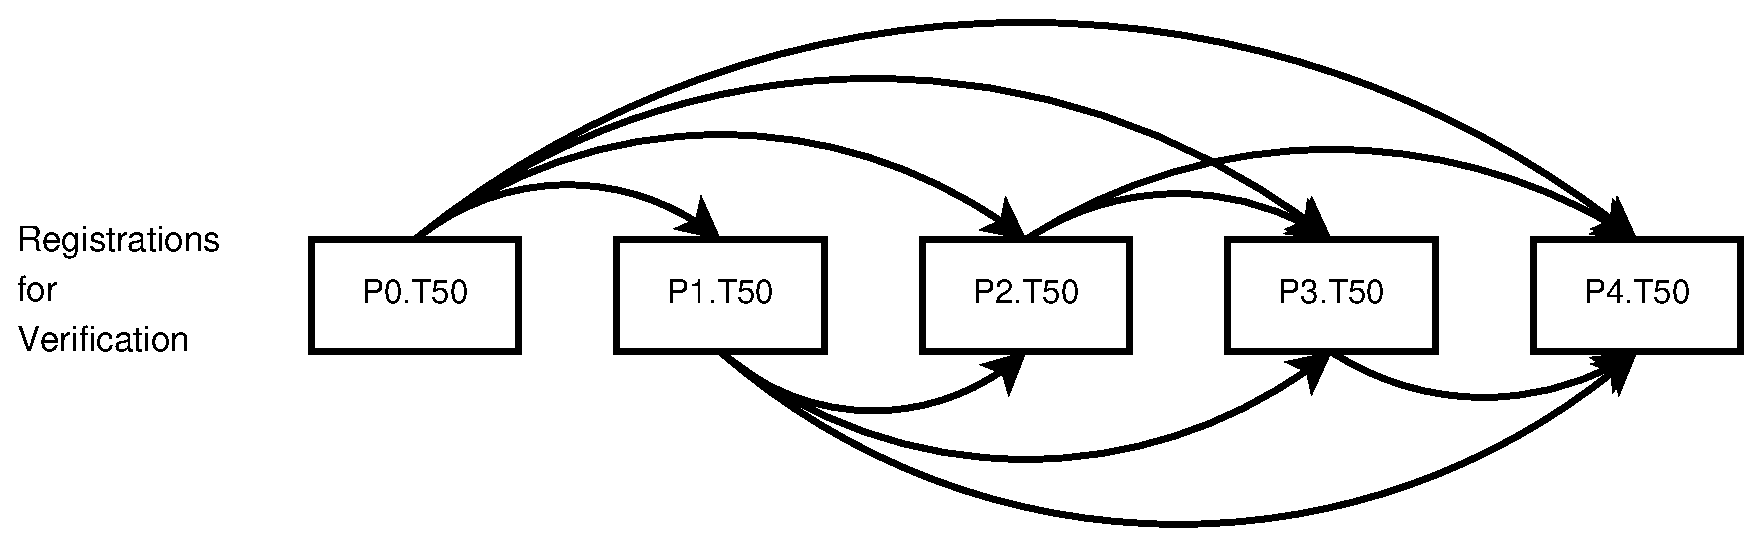
\includegraphics[width=5in]{registrations_for_validation}
%\includegraphics[width=4in]{"registrations-training"}
%\includegraphics[width=4in]{"registrations-validation"}
%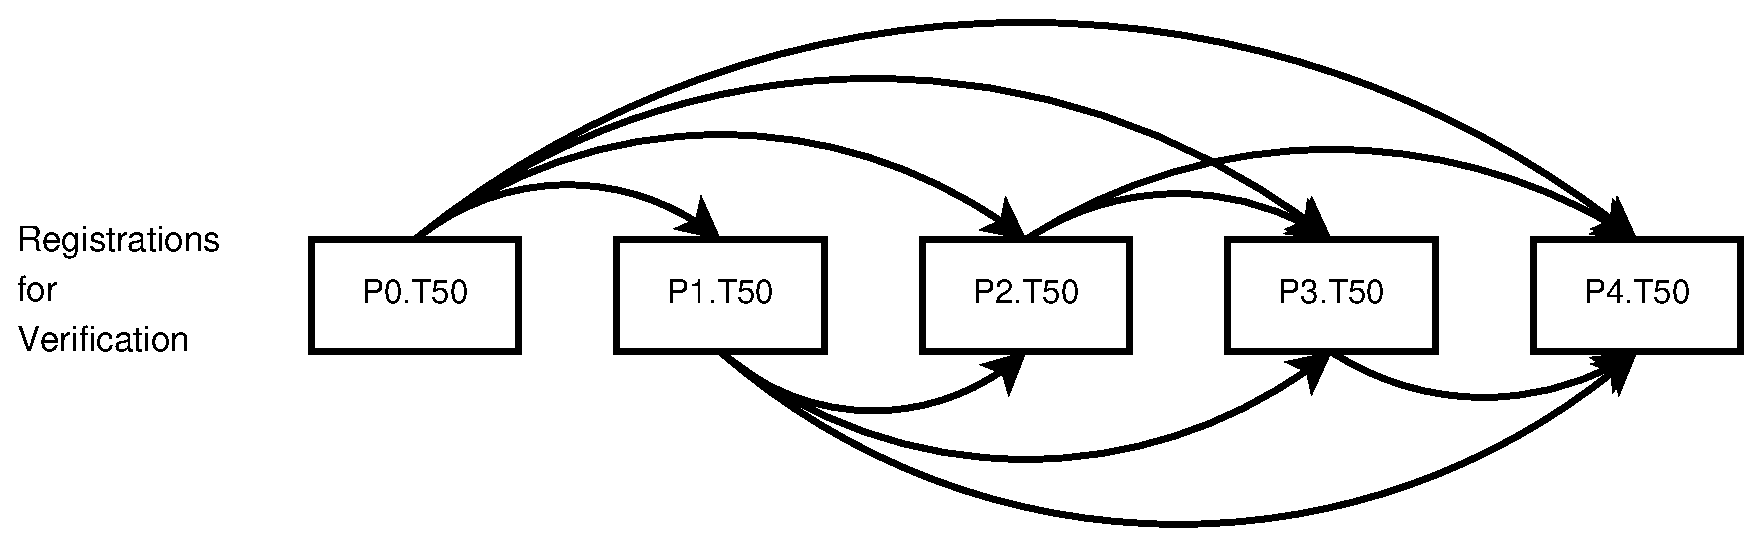
\includegraphics[width=5in]{registrations_for_validation}
\end{center}
\caption{Registration schemes used for training (above) and verification (below). An arrow from P\textit{A}.T\textit{X} to P\textit{B}.T\textit{Y} means registering the image of patient \textit{A} at time \textit{X} to the image of patient \textit{B} at time \textit{Y}.}
\label{fig:testing_schemes}
\end{figure}

We used Mutual Information \cite{Mattes03:TMI} as the similarity metric in
both registration levels. The similarity registrations used about $1\%$ of
voxels from the liver region for metric calculation, and were executed for
150 iterations. The B-spline deformation registrations used about $3\%$ of
voxels, and were executed for 50 iterations. A $7 \times 7 \times 7$ B-spline
control grid over the liver region was used to model the tissue deformations.

We studied the behaviors of the proposed method using each of the three optimization algorithms described above, and used the parameters suggested in the ITK examples, which were $(1.0,0.001,10,0.7)$, as a reference for comparison.
For PSO, 25 particles were used and 30 generations were executed. It does not need an initial value of the parameters; instead, the bounding region $(0.5,0.0001,0.1,0.1)-(2.0,0.01,100,0.9)$ was used to create the particles as well as to constrain the parameters during the optimization.
For CMA-ES, $(1.0,0.01,50,0.5)$ was used as the initial value, 7 particles were used in each iteration, and 100 total iterations were performed.
For adapted BF, we placed a $5 \times 5 \times 5 \times 5$ grid over the same bounding region used for the PSO and performed function evaluations at all grid points, then an additional optimization with the downhill simplex algorithm was performed for 50 iterations. Each of the above experiments performed about 700 total registrations, which were executed in  parallel using 10 slave processes.

We used a cluster of four computers and the MPICH2 implementation of the MPI protocol to perform the experiments. Each computer was equipped with an Intel i7 CPU, 12GB RAM and 64-bit Windows 7. One computer executed the master process plus one slave process, and the rest of the workstations executed three slave processes each. For each optimization algorithm being studied, the computation took about 8 hours.

\subsection{Results and Discussion}

We first look at the function plots at the ITK suggested value and along each parameter axis. From Fig.~\ref{fig:f_plots}, it is obvious that we were dealing with a function that has many local minima, and searching for an optimal solution is challenging.

%============================================
\begin{figure}[tb!]
\begin{center}
\begin{tabular}{cc}
\includegraphics[width=2.5in]{cf_plot_p0} &
\includegraphics[width=2.5in]{cf_plot_p1} \\
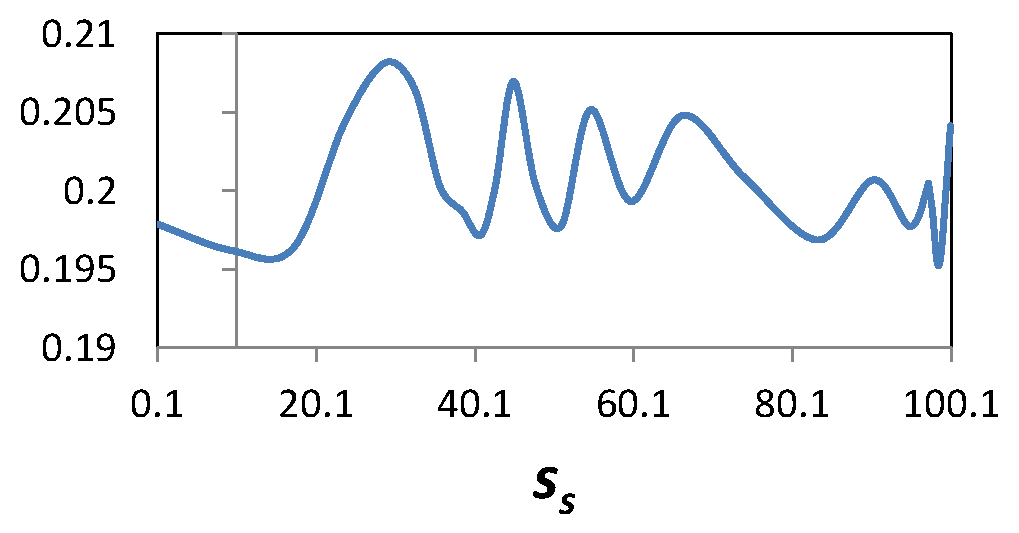
\includegraphics[width=2.5in]{cf_plot_p2} &
\includegraphics[width=2.5in]{cf_plot_p3} \\
\end{tabular}
\end{center}
\caption{Function plots along each parameter axis in the bounded feasible region used for the PSO algorithm. Vertical lines in the middle show the locations of individual components of the ITK recommended value.}
\label{fig:f_plots}
\end{figure}

%============================================
\begin{figure}[!b]
\begin{center}
%\includegraphics[width=6in]{results_training_plot}
\includegraphics[width=6in]{results_training_2}
\end{center}
\caption{Overall alignments over time for the three optimization algorithms. The value for the adapted BF was available only at the end of the optimization. This value as well as the ITK suggested one is displayed for illustration purposes.}
\label{fig:results_training}
\end{figure}

Fig.~\ref{fig:results_training} shows the overall alignments over time for the three optimization algorithms being studied, and Table~\ref{tab:results_validation} shows the final alignments when the obtained parameters were used to register the testing images.
In Fig.~\ref{fig:results_training}, all three studied optimization algorithms were able to improve the overall alignments at the end of optimizations for the training images, with the best result being produced by PSO.
From Table~\ref{tab:results_validation}, we observed an overall $2\%$ improvement in final alignment for PSO, and $1\%$ for adapted BF when the obtained parameters were applied to the testing images. No improvement was observed for CMA-ES, but the results were still comparable to those obtained using the ITK suggested value. We believe that the CMA-ES results can be further improved if we allow more iterations and use the improved CMA-ES implementations that incorporate anisotropic initialization for different parameters.

%============================================
\begin{table}[t!]
\caption{Results with testing images: final alignments (complemented DSC) obtained from parameters suggested by ITK and our proposed method. An arrow from P\textit{A}.T\textit{X} to P\textit{B}.T\textit{Y} means registering the image of patient \textit{A} at time \textit{X} to the image of patient \textit{B} at time \textit{Y}.}
\label{tab:results_validation}
\begin{center}
%
\begin{tabular}{c|c|c|c|c}
\hline
Registration & ITK suggested & PSO & CMA-ES & Adapted BF \\
\hline \hline
P0.T50 $\rightarrow$ P1.T50 & 0.24 & 0.24 & 0.26 & 0.24 \\
\hline
P0.T50 $\rightarrow$ P2.T50 & 0.13 & 0.11 & 0.15 & 0.12 \\
\hline
P0.T50 $\rightarrow$ P3.T50 & 0.13 & 0.10 & 0.13 & 0.12 \\
\hline
P0.T50 $\rightarrow$ P4.T50 & 0.22 & 0.22 & 0.21 & 0.20 \\
\hline
P1.T50 $\rightarrow$ P2.T50 & 0.21 & 0.16 & 0.20 & 0.15 \\
\hline
P1.T50 $\rightarrow$ P3.T50 & 0.14 & 0.14 & 0.17 & 0.17 \\
\hline
P1.T50 $\rightarrow$ P4.T50 & 0.22 & 0.24 & 0.22 & 0.22 \\
\hline
P2.T50 $\rightarrow$ P3.T50 & 0.19 & 0.14 & 0.21 & 0.16 \\
\hline
P2.T50 $\rightarrow$ P4.T50 & 0.16 & 0.15 & 0.18 & 0.16 \\
\hline
P3.T50 $\rightarrow$ P4.T50 & 0.23 & 0.23 & 0.24 & 0.23 \\
\hline \hline
mean $\pm$ std.dev. & 0.19 $\pm$ 0.04 & 0.17 $\pm$ 0.05 & 0.20 $\pm$ 0.04 & 0.18 $\pm$ 0.04 \\
\hline
\end{tabular}
%
\end{center}
\end{table}

We also examined the parameters produced by the three algorithms. We observed that the optimal value produced by PSO, $(0.5, 0.001, 0.1, 0.1)$, was quite different from the ITK suggested one. This is reasonable as we can see from Fig.~\ref{fig:f_plots} that the function was very noisy and multiple local minima existed.

\section{Conclusion}

In this paper we presented a framework to automate the process of system parameters tuning, and used it to refine the internal parameters of a common registration task. The proposed approach is more intuitive and systematic than the conventional trial-and-error approach, and was able to produce improved system parameters. We also proposed an MPI-based implementation such that the expensive tuning task can be performed using a cluster of workstations.

Future work includes additional evaluation with different data modalities and data with more variability. We will also improve the MPI implementation to enable automatic load balancing to further improve computation performance.

%%%%%%%%%%%%%%%%%%%%%%%%%%%%%%%%%%%%%%%%%%%%%%%%%%%%%%%%%%%%%
\acknowledgments     %>>>> equivalent to \section*{ACKNOWLEDGMENTS}

This work was supported by NLM/NIH contract HHSN276201000578P.

%%%%%%%%%%%%%%%%%%%%%%%%%%%%%%%%%%%%%%%%%%%%%%%%%%%%%%%%%%%%%
%%%%% References %%%%%

\bibliography{rhgong_atosp}   %>>>> bibliography data in report.bib
\bibliographystyle{spiebib}   %>>>> makes bibtex use spiebib.bst

\end{document}
